%%
% Report of my internship.
% It has to give an introduction to the context and explain my work.
%%
\documentclass[12px]{article}

\usepackage[noend]{algpseudocode}
\usepackage[english]{babel}
\usepackage[a4paper]{geometry}
\usepackage[hidelinks]{hyperref}

\usepackage{algorithm}
\usepackage{apacite}
\usepackage{stmaryrd}
\usepackage{tikz}
\usepackage{todonotes}
\usepackage{wrapfig}


\begin{document}
  \section{Introduction}
    % Some bullshit is expected here I guess ?
    % Goal of the internship (maybe quickly as not everything is supposed to be introduced)
    % Technical informations about the internship, team, ...

  \section{Context and state of the art}
    % Give any information about what isn't my work
    \subsection{Union-Find algorithms}
      \subsubsection{Disjoint set structure}
        % Definition of a disjoint set structure
        The disjoint set structure is a very classical structure that represents a partition of a finite set $X = \biguplus\limits_{i \in I} S_i$. It is meant to allow three fast queries:
        \begin{itemize}
          \item $\Call{makeset}{x}$: add the element $x$ to the structure, initially in a singleton.
          \item $\Call{Union}{x, y}$: alter the structure to merge the set $x$ belongs to and the set $y$ belongs to. After such an operation, $\exists! i \in I~/~x \in S_i \land y \in S_i$.
          \item $\Call{find}{x}$: give a unique representative of the set $x$ belongs to. It means that $\forall x, y \in X,~\Call{find}{x} = \Call{find}{y} \Leftrightarrow \exists! i \in I~/~x \in S_i \land y \in S_i$.
        \end{itemize}

        In practice, it is usually represented by a forest of the elements of $X$, $\textsc{makeset}$ builds a tree containing only its root, $\textsc{union}$ merges two trees and $\textsc{find}$ returns the root of a tree given one of its nodes.
        In a program, such a forest is represented by an array of size $|X|$, assuming that $X = \llbracket 0, |X|-1 \rrbracket$, the element of index $x$ will be $y$ if $y$ is the parent of $x$ in a tree, or $x$ if $x$ is a root.

        In order to lighten notations, whenever such a structure is used, we note the parent of any node $x$ as $p(x)$.

        \begin{figure}[h]
          \caption{A disjoint set structure representing $\{\{0, 1, 2\}, \{3\}, \{4, 5\}\}$}
          \centering
          \vspace{0.2cm}
          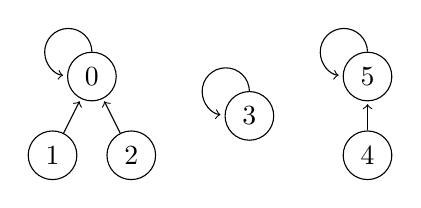
\begin{tikzpicture}[shorten >=1pt]
            \tikzstyle{vertex} = [circle, draw=black]
            \tikzstyle{legend} = [color=gray, font=\tiny]

            \node[vertex] (0) at (1, 1) {$0$};
            \node[vertex] (1) at (0.5, 0) {$1$};
            \node[vertex] (2) at (1.5, 0) {$2$};
            \node[vertex] (3) at (3, 0.5) {$3$};
            \node[vertex] (4) at (4.5, 0) {$4$};
            \node[vertex] (5) at (4.5, 1) {$5$};

            \draw [->] (0.90) arc (1:264:3mm) {};
            \draw [->] (3.90) arc (1:264:3mm) {};
            \draw [->] (5.90) arc (1:264:3mm) {};

            \draw [->] (1) -- (0);
            \draw [->] (2) -- (0);
            \draw [->] (4) -- (5);
          \end{tikzpicture}
          \hspace{1cm}
          \raisebox{0.5cm}{
            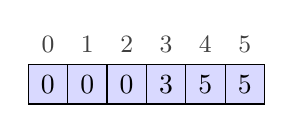
\begin{tikzpicture}[shorten >=1pt]
              \tikzstyle{value} = [draw=black, fill=blue!15, minimum width=0.5cm, minimum height=0.5cm]
              \tikzstyle{index} = [color=darkgray, font=\small]

              \foreach \i / \x in {0/0, 1/0, 2/0, 3/3, 4/5, 5/5} {
                \node[index] at (\i / 2, 0.5) {\i};
                \node[value] at (\i / 2, 0) {\x};
              }

            \end{tikzpicture}
          }
        \end{figure}

      \subsubsection{Classical union-find algorithm}
        % Classical th. implementation of union-find, explaination why (th. complexity), applications ?
        \setlength\intextsep{0pt}
        \begin{wrapfigure}{r}{5.6cm}
          \centering
          \begin{minipage}{\linewidth}
            \begin{algorithm}[H]
              \caption{General structure of Union-Find}
              \label{alg:union-find}
              \begin{algorithmic}[1]
                \State $F \gets \emptyset$
                \ForAll {$x \in V$}
                  \State \Call{makeset}{x}
                \EndFor
                \ForAll {$(x, y) \in E$}
                  \If {$\Call{find}{x} \neq \Call{find}{y}$}
                    \State $\Call{union}{x, y}$
                    \State $F \gets F \cup \{x, y\}$
                  \EndIf
                \EndFor
              \end{algorithmic}
            \end{algorithm}
          \end{minipage}
        \end{wrapfigure}

        A very typical application of this structure is to find a spaning forest for an undirected graph. A general algorithm used to answer this problem is called \emph{union-find} (alg. \ref{alg:union-find}).

        Typically, \textsc{find} runs over the tree until it reaches the root, keeps track of every nodes on the path and finally set their parent to be the root. In this case \textsc{union} doesn't need to compress the trees and will just make one of the roots be parent of the other, the new root can be chosen arbitrary or given a criteria (index, rank, ...).

        This algorithm can actualy be implemented with many variations (\citeA{ufexp10}), where a typical goal is to make sure that trees never get too high, thus compressing the path leading to the root while processing \textsc{find} operation.


      \subsubsection{REM algorithm}
        % Definition and analysis of REM, explaination on why it is awesome
        \todo[noline,color=green!30,inline]{Add a reference to \emph{Dijkstra, E.W.: A Discipline of Programming} ?}

        \setlength\intextsep{0pt}
        \begin{wrapfigure}{r}{5cm}
          \centering
          \begin{minipage}{\linewidth}
            \begin{algorithm}[H]
              \caption{Rem's algorithm}
              \label{alg:rem}
              \begin{algorithmic}[1]
                \State $r_x \gets x, r_y \gets y$
                \While {$p(r_x) \neq p(r_y)$}
                  \If {$p(r_x) > p(r_y)$}
                    \If {$r_x = p(r_x)$}
                      \State $p(r_x) \gets p(r_y)$
                      \State \Return false
                    \EndIf
                    \State $p_{r_x} \gets p(r_x)$
                    \State $p(r_x) \gets p(r_y)$
                    \State $r_x \gets p_{r_x}$
                  \Else
                    \If {$r_y = p(r_y)$}
                      \State $p(r_y) \gets p(r_x)$
                      \State \Return false
                    \EndIf
                    \State $p_{r_y} \gets p(r_y)$
                    \State $p(r_y) \gets p(r_x)$
                    \State $r_y \gets p_{r_y}$
                  \EndIf
                \EndWhile
                \State \Return true
              \end{algorithmic}
            \end{algorithm}
          \end{minipage}
        \end{wrapfigure}

        A familly of variation, called \emph{interleaved algorithms} in \citeA{ufexp10} replaces the two separate find operations at line 5 of Union-Find (alg. \ref{alg:union-find}). This kind of algorithm will instead operate by running over the forest simultaneously from the two starting nodes. The first advantage of this kind of algorithm is that it won't need to reach both roots on every case.

      In Rem's algorithm, line 5 and 6 of algorithm \ref{alg:union-find} are replaced by algorithm \ref{alg:rem} which handles find operations, merging components if they are disconnected and compression in one loop.

      \todo[color=blue!30,fancyline]{Quick complexity review}

    \subsection{Distributed algorithms}
      % Introduction to distributed algorithmic, existing implementation

    \subsection{Shared algorithms}
      % Introduction to shared algorithmic, existing implementation


  \section{Writing REM as a distributed memory algorithm}
    % Description of the algorithm, experimental results


  \section{Mixing up distributed and shared algorithms}
    % Description of parallelized parts, experimental results


  \section{Conclusion}


  \section{Appendices}
    % Proofs, maybe extra datas
    \citeA{ufdist09}
    \citeA{ufexp10}


  \bibliographystyle{apacite}
  \bibliography{references}
\end{document}
